\documentclass[border=10pt]{standalone}

\usepackage{tikz}
\usepackage{tikzsymbols}
\usetikzlibrary{calc,patterns,shapes.geometric}

\def\centerarc[#1](#2)(#3:#4:#5){\draw[#1] ($(#2)+({#5*cos(#3)},{#5*sin(#3)})$) arc (#3:#4:#5);}

\begin{document}
	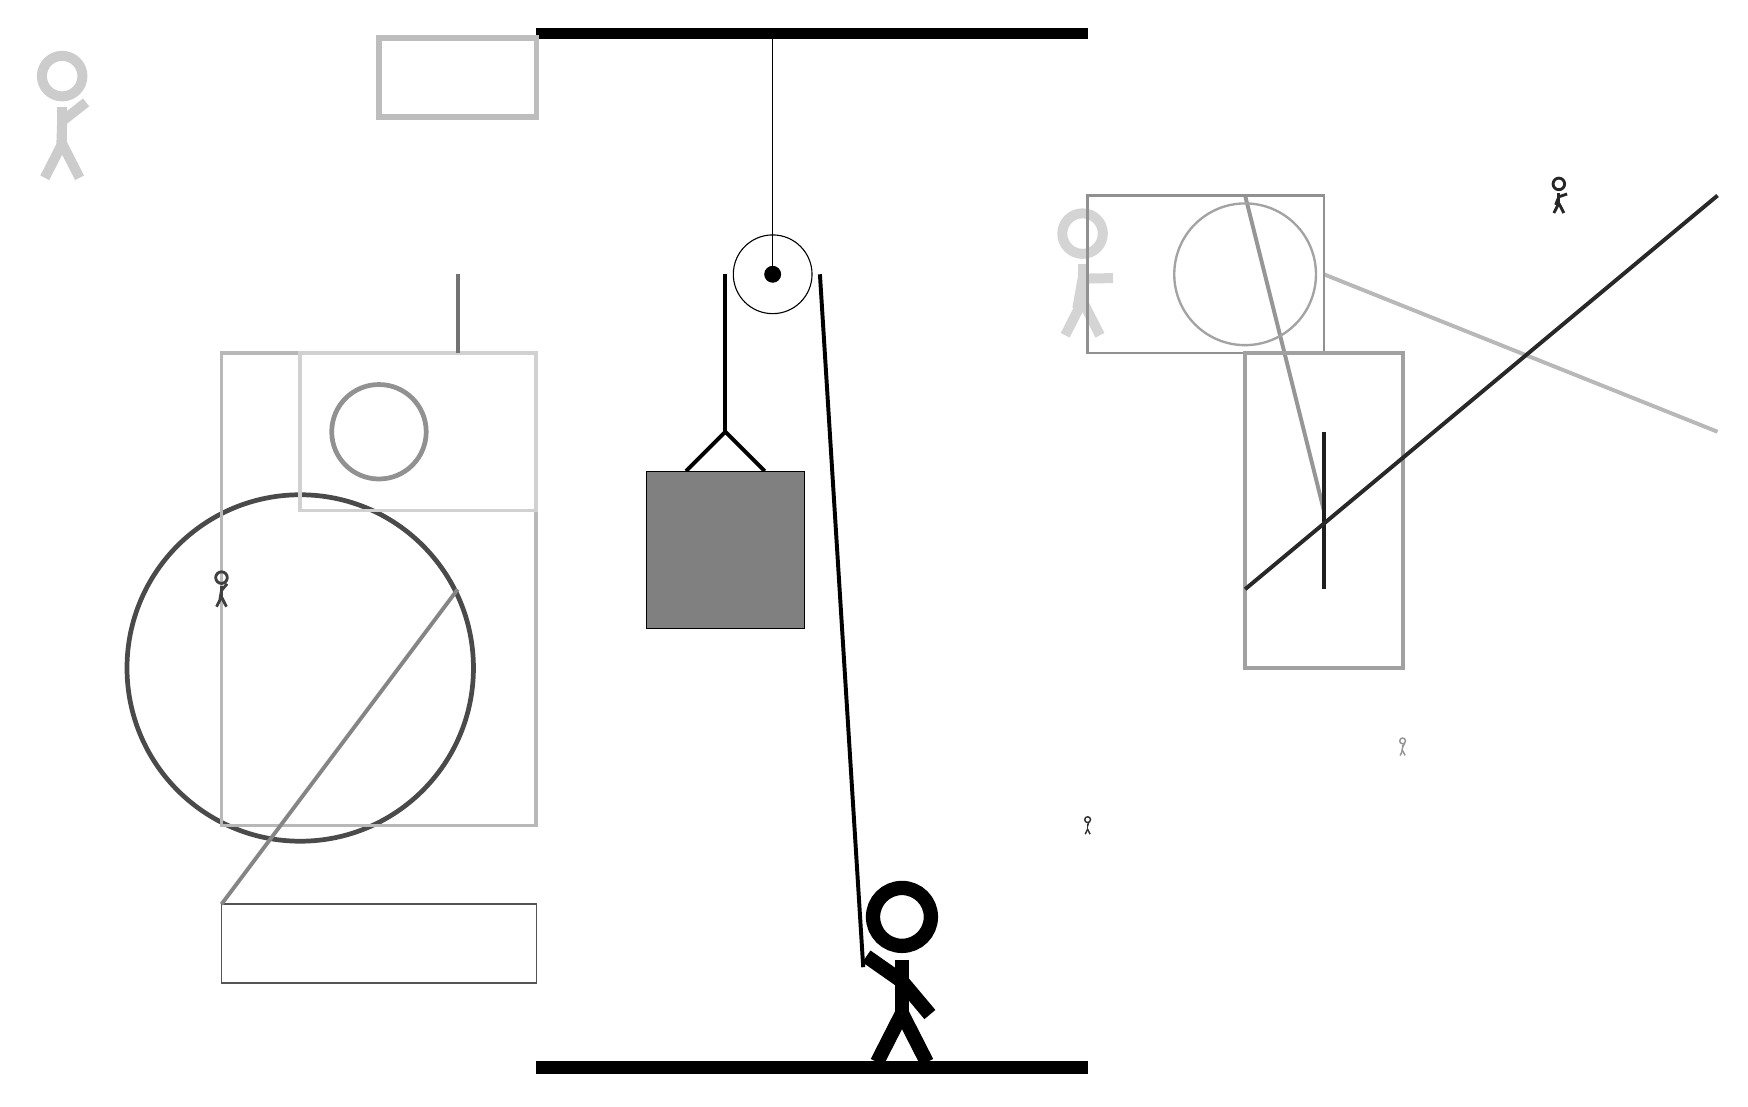
\begin{tikzpicture}
		%%%%% START %%%%%
		
		\draw[fill=black] (-2, 10) rectangle (5, 10.125);
		
		\draw (1, 7) circle (0.5);
		\draw[fill=black] (1, 7) circle (0.1);
		\draw (1, 10) -- (1, 7);
		
		\node[line width=0.5mm, color=black!17] at (5, 7) {\Strichmaxerl[7][80][1]};
		
		\draw [line width=0.6mm, color=black!71](-5, 2) circle (2.2);
		\draw[line width=0.5mm, color=black!28](8, 7) -- (13, 5);
		\draw[line width=0.5mm, color=black!41](7, 8) -- (8, 4);
		\node[line width=0.7mm, color=black!81] at (5, 0) {\Strichmaxerl[1][90][75]};
		
		\draw[line width=0.3mm, color=black!43] (5, 6) rectangle (8, 8);
		\draw[line width=0.5mm, color=black!88](8, 3) -- (8, 5);
		\draw[line width=0.5mm, color=black!28] (-2, 0) rectangle (-6, 6);
		\draw[line width=0.5mm, color=black!37] (7, 2) rectangle (9, 6);
		
		\draw [line width=0.3mm, color=black!36](7, 7) circle (0.9);
		\draw[line width=0.2mm, color=black!67] (-2, -1) rectangle (-6, -2);
		\draw[line width=0.5mm, color=black!18] (-2, 4) rectangle (-5, 6);
		\draw[line width=0.7mm, color=black!26] (-2, 10) rectangle (-4, 9);
		\draw [line width=0.6mm, color=black!43](-4, 5) circle (0.6);
		\draw[line width=0.5mm, color=black!84](7, 3) -- (13, 8);
		\node[line width=0.5mm, color=black!20] at (-8, 9) {\Strichmaxerl[7][88][38]};
		\draw[line width=0.5mm, color=black!48](-6, -1) -- (-3, 3);
		
		\node[line width=0.3mm, color=black!75] at (-6, 3) {\Strichmaxerl[2][80][50]};
		\node[line width=0.6mm, color=black!85] at (11, 8) {\Strichmaxerl[2][68][19]};
		\draw[line width=0.5mm, color=black!55](-3, 7) -- (-3, 6);
		\node[line width=0.4mm, color=black!42] at (9, 1) {\Strichmaxerl[1][80][63]};
		
		
		\draw[line width=0.5mm] (-0.1, 4.5) -- (0.4, 5.0) -- (0.9, 4.5);
		\draw[fill=black!50] (-0.6, 4.5) rectangle (1.4, 2.5);
		
		\draw[line width=0.5mm] (0.4, 7) -- (0.4, 5.0);
		\centerarc[line width=0.5mm](1, 7)(0:180:0.6);
		\draw[line width=0.5mm](1.6, 7) -- (2.15, -1.8);
		
		\node at (2.6, -1.9) {\Strichmaxerl[10][-35][-50]};
		
		\draw[fill=black] (-2, -3) rectangle (5, -3.15);
		
		%%%%% END %%%%%
	\end{tikzpicture}
\end{document}